\subsubsection{Implementation}\label{subsection:license-amazon-implementation}
%START TEXT INPUT
This is my real text! Rest might be copied or not be checked!
%START TEXT INPUT

%
different approach to perform license verification and enforce result
google lvl include and integrate modified version of lvl library, not required to implement any mechanism on their own, done by amazon packaging tool
when submitting can check amazon DRM (see picture), applay amazon DRm to "Protect your application from unauthorized use. Without DRM, your app can be used without restrictions by any user."
"As part of the ingestion process Amazon removes your developer signature and applies an Amazon signature. This signature is unique to you, does not change, and is the same for all apps in your account." so developer signing the application by the develoepr before submitting is not necessary, amazon decompiles apk, injects drm code, compiles it and signs it with the "amazon developer" certificate

no sample implementation to add by developer but inject own logic in each app (same for every app)
\cite{munteanLicense}
%

\begin{figure}[h]
    \centering
    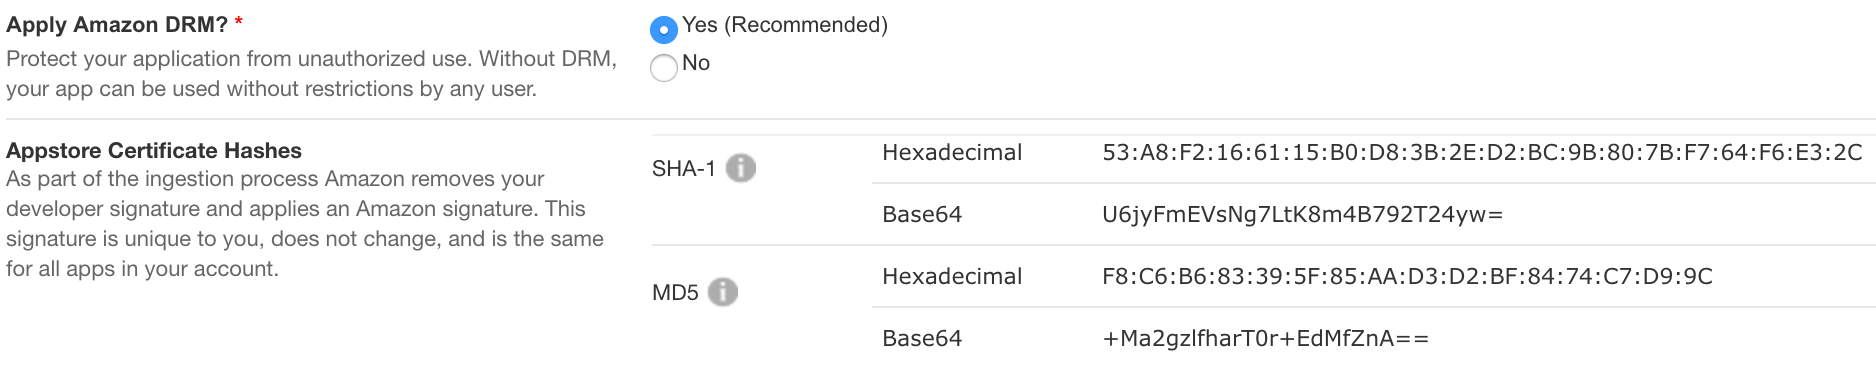
\includegraphics[width=0.8\textwidth]{data/amazon.png}
    \caption{amazon}
    \label{fig:amazon}
\end{figure}


\lstinputlisting[
  basicstyle=\footnotesize,
  breakatwhitespace=false,
  breaklines=true,
  captionpos=b,
  frame=single,
  numbers=left,
  language=Java,
  linerange={77-80},
  firstnumber=77,
  caption={Callback},
  label={lst:lvlcallback}
]{data/amazon.java}

rename onCreate to onCreateMainActivity
start in new onCreate         Kiwi.onCreate((Activity) this, true);
